\documentclass{standalone}
\usepackage{tikz}
\usepackage{ctex,siunitx}
\setCJKmainfont{Noto Serif CJK SC}
\usepackage{tkz-euclide}
\usepackage{amsmath}
\usepackage{wasysym}
\usetikzlibrary{patterns, calc}
\usetikzlibrary {decorations.pathmorphing, decorations.pathreplacing, decorations.shapes,}
\begin{document}
\small
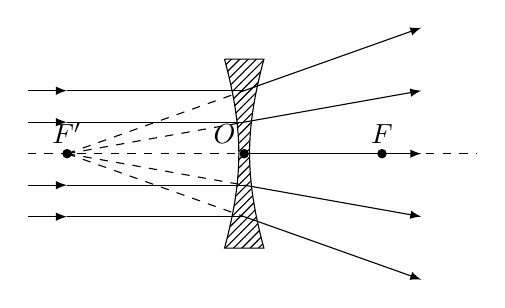
\begin{tikzpicture}[>=latex,scale=1.0]
  \useasboundingbox(-2.5,-1.6)rectangle(3.2,1.6);
  \draw [pattern=north east lines] (0,1.2) to [bend left=15] (0,-1.2)--(.5,-1.2) to [bend left=15](.5,1.2)--(0,1.2);
  \draw [dashed] (-2.5,0)--(3.2,0);
\node at (-2,0) [above]{$F'$};
\node at (2,0) [above]{$F$};
\draw (-2,0)[fill=black] circle (1.5pt);    \draw (2,0)[fill=black] circle (1.5pt);
\foreach \x in {-.8,-.4,.4,.8}
  {
      \draw[->] (-2.5,\x)--(-2,\x);
      \draw[dashed](-2,0)--(0.25,\x);
      \draw[->](0.25,\x)--(2.5,2*\x);
  }  
  \draw  (-2,-.8)--(0.25,-.8)    ;
  \draw  (-2,-.4)--(0.25,-.4)    ;
  \draw  (-2,.4)--(0.25,.4)    ;
  \draw  (-2,.8)--(0.25,.8)    ;
  \draw[->](0.25,0)--(2.5,0);
 \node at (0,0)[above] {$O$};
 \draw (0.25,0)[fill=black] circle (1.5pt);
\end{tikzpicture}
\end{document}